% !TEX root = ../thesis.tex

\chapter{Methodology} \label{chp:methodology}

\section{The Three-Tier Digital Twin Framework}

This research introduces a novel classification framework for Digital Twin environments based on decision-making complexity rather than traditional engineering maturity metrics. The framework establishes three distinct tiers that reflect the evolutionary progression of cognitive reasoning requirements in physical world applications.

\begin{figure}[htbp]
\centering
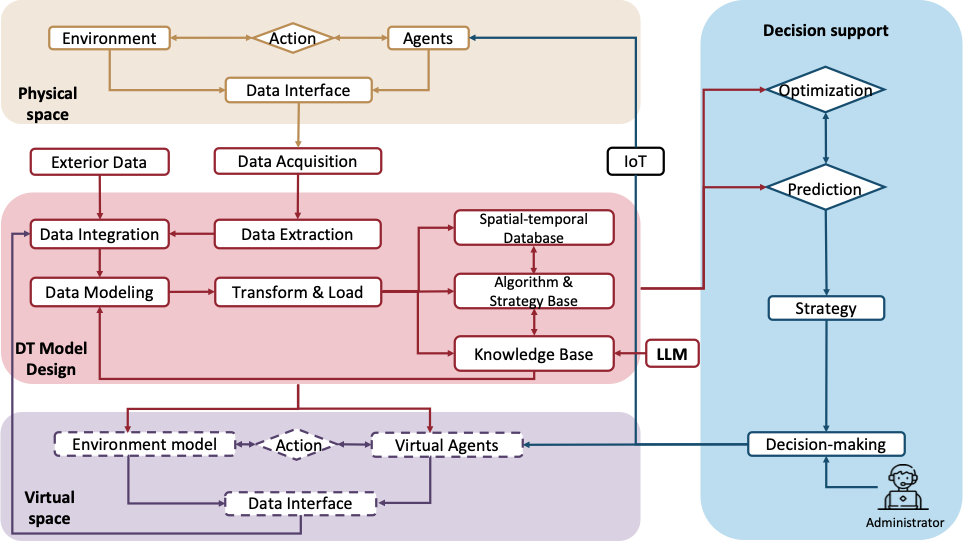
\includegraphics[width=0.9\textwidth]{Framework/DT_Framework.png}
\caption{Three-Tier Digital Twin Framework showing the progression from L1 Descriptive Twins through L2 Predictive Twins to L3 Interactive Twins, with corresponding cognitive complexity requirements.}
\label{fig:dt_framework}
\end{figure}

The framework structure builds upon the observation that different physical decision-making contexts impose fundamentally different cognitive requirements on reasoning systems. Rather than focusing solely on technical implementation details, this classification emphasizes the type and complexity of reasoning required for effective system operation.

\begin{table}[h]
\centering
\caption{Three-Tier Digital Twin Framework}
\label{tab:three_tier_framework}
\begin{tabular}{llll}
\toprule
\textbf{Tier} & \textbf{Type} & \textbf{Decision Mode} & \textbf{Case Study} \\
\midrule
L1 & Descriptive Twin & Diagnostic (What is?) & Building Monitoring \\
L2 & Predictive Twin & Strategic (What if?) & Medical Diagnosis \\
L3 & Interactive Twin & Actionable (What to do?) & UAV Navigation \\
\bottomrule
\end{tabular}
\end{table}

L1 - Descriptive Twin represents the foundational tier focused on understanding current system states through comprehensive data integration and analysis. These environments serve as the "authoritative record of reality" by maintaining up-to-date representations of physical system conditions based on multiple information sources including sensor data, historical records, and documentation.

The key challenges of L1 environments lie in information fusion and noise processing, directly testing the data grounding and robustness of the perception module. The complexity arises from the need to handle heterogeneous data integration, which involves combining structured databases, time-series sensor data, and unstructured text documents while maintaining semantic coherence \cite{lu2020digital}. Temporal alignment presents additional challenges as data from different sources must be synchronized despite varying sampling rates and timestamps. Quality assessment requires identifying and handling inconsistent, missing, or corrupted data across multiple sources. Finally, semantic mapping involves translating natural language queries into appropriate database queries, API calls, and file operations.

L1 environments provide ideal testing grounds for DT-RAG (Digital Twin Retrieval-Augmented Generation) capabilities, as they require sophisticated information retrieval and synthesis without the complexity of predictive modeling or real-time control. The cognitive demands focus on comprehensive understanding of current conditions rather than future planning or action execution.

L2 - Predictive Twin extends beyond descriptive capabilities to function as a "causal simulator of time" that can explore potential future scenarios through sophisticated modeling and simulation. These environments enable strategic reasoning about possible outcomes and their implications for decision-making.

The key challenges of L2 environments lie in complex model orchestration and semantic understanding of inputs/outputs, directly testing the planning and tool utilization capabilities of the reasoning module. The complexity includes model selection, which involves choosing appropriate simulation models from available options based on specific prediction requirements. Parameter configuration requires understanding complex input requirements and generating appropriate configuration files for simulations. Execution management involves coordinating potentially long-running simulations while maintaining system responsiveness. Result interpretation demands extracting meaningful insights from complex simulation outputs, often requiring domain expertise.

L2 environments demand sophisticated reasoning capabilities that go beyond simple information retrieval to include hypothesis formation, experimental design, and causal inference. The cognitive architecture must be capable of understanding complex model interfaces, generating appropriate inputs, and interpreting results in ways that support strategic decision-making.

L3 - Interactive Twin represents the most complex tier, functioning as a "counterfactual sandbox for action" where decisions have immediate consequences in real-time environments. These systems must balance multiple objectives while maintaining safety and effectiveness under dynamic conditions.

The key challenges of L3 environments lie in the trade-offs and assurance among safety, task efficiency, and real-time performance, directly testing the effectiveness of the dual-loop safety execution mechanism of the action module. The complexity encompasses real-time constraints that require making decisions within strict time limits while maintaining safety and effectiveness. Safety assurance involves ensuring all actions remain within safe operational boundaries despite uncertainties. Adaptive planning requires modifying plans based on real-time feedback and changing environmental conditions. Multi-objective optimization involves balancing competing objectives such as task completion, safety, and resource efficiency.

L3 environments represent the ultimate test of cognitive architecture capabilities, requiring integration of perception, reasoning, and action modules in real-time scenarios where errors can have serious consequences. The system must demonstrate not only intelligent reasoning but also robust safety mechanisms and adaptive capabilities.

The framework's effectiveness is demonstrated through its ability to provide standardized evaluation environments across different complexity levels, enable systematic comparison of different architectural approaches, support incremental capability development and testing, and facilitate reproducible research through well-defined experimental conditions.

This classification framework addresses a critical gap in current Digital Twin evaluation approaches by focusing on cognitive complexity rather than purely technical metrics. It provides a foundation for systematic evaluation of LLM-CPS integration approaches and enables researchers to develop and validate capabilities in a structured, progressive manner.

\section{CORTEX: A Cognitive Architecture for LLM-driven Agents}

CORTEX (Cognitive Operations for Real-Time EXecution) represents a systematic architectural approach to integrating LLM reasoning capabilities with Digital Twin environments. The architecture addresses the three fundamental challenges of LLM-physical world integration through specialized modules designed for perception, reasoning, and action.

\begin{figure}[htbp]
\centering
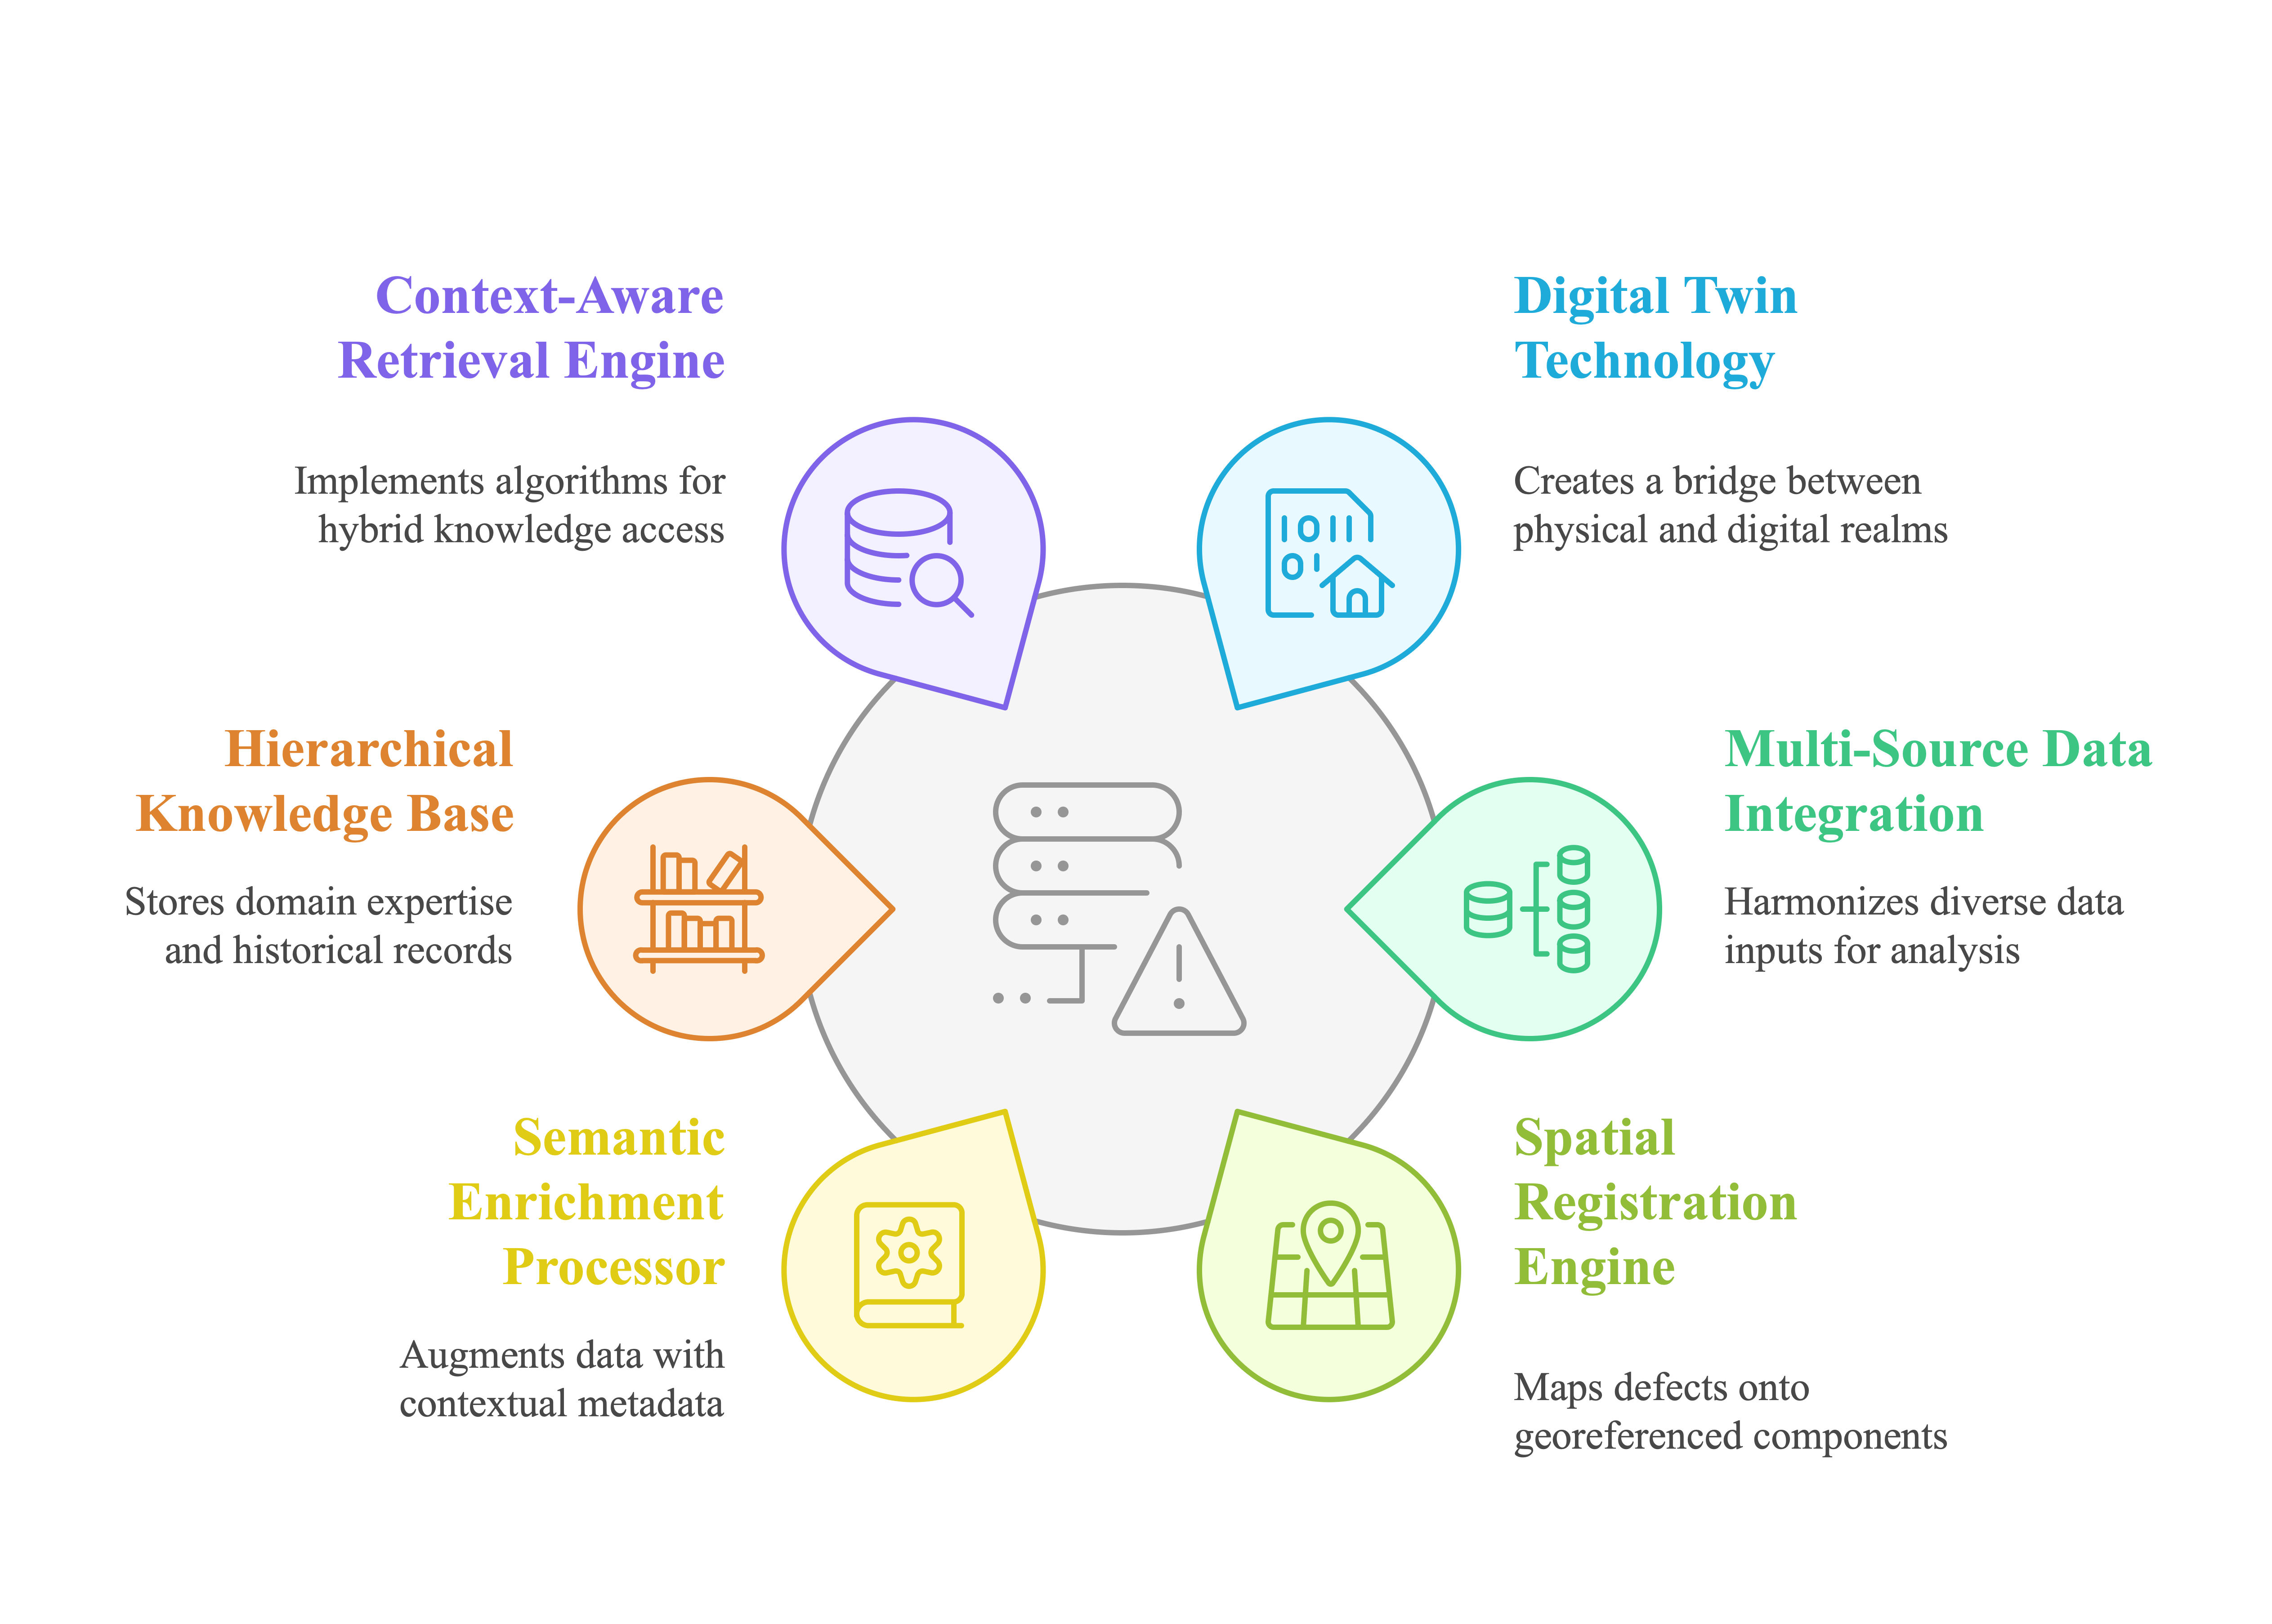
\includegraphics[width=0.9\textwidth]{DefectGPT/Overall Framework.png}
\caption{CORTEX Architecture Overview showing the three main modules (Perception, Reasoning, Action) and their interfaces with the three-tier Digital Twin environment.}
\label{fig:architecture_overview}
\end{figure}

The architectural design philosophy emphasizes modularity, allowing different components to be developed, tested, and upgraded independently while maintaining systematic integration across the entire system. This approach enables targeted solutions to specific challenges while ensuring comprehensive coverage of LLM-CPS integration requirements.

Digital Twin-native Retrieval-Augmented Generation (DT-RAG) represents a fundamental extension of traditional RAG architectures specifically designed for the heterogeneous, multi-modal data environments typical of Digital Twins. Unlike conventional RAG systems that primarily handle text-based knowledge, DT-RAG must integrate structured databases, time-series sensor data, and unstructured documents while maintaining real-time responsiveness.

The process begins with a natural language information requirement generated by the Reasoning Module. The DT-RAG intent analyzer first parses this requirement and decomposes it into multiple sub-tasks. Subsequently, these sub-tasks are distributed to a parallel suite of specialized data adapters for execution. The structured data adapter converts intentions into SQL statements to query asset databases, handling complex joins and aggregations across multiple tables \cite{scholak2021duorat}. The time-series adapter generates specialized queries to extract sensor readings from time-series databases, including temporal filtering and statistical aggregations \cite{yue2022ts2vec}. The document retrieval adapter utilizes traditional vector retrieval to search for relevant text within unstructured documents, employing semantic similarity matching and keyword-based filtering \cite{karpukhin2020dense}.

The heterogeneous results returned by these parallel queries require sophisticated fusion mechanisms. The most critical step in DT-RAG is integrating these information fragments into a unified, context-rich textual summary. This fusion process involves semantic alignment to ensure that information from different sources refers to the same physical entities or phenomena. Temporal synchronization aligns data from different time periods and sampling rates into coherent temporal narratives. Quality weighting assigns confidence scores to different information sources based on reliability and relevance. Contextual summarization generates natural language summaries that preserve essential quantitative relationships while being optimized for LLM comprehension.

The output is a comprehensive textual representation that maintains the richness of heterogeneous Digital Twin data while being optimized for LLM processing. This approach enables LLMs to reason effectively about physical systems without requiring fundamental changes to model architectures or training procedures.

Model-Profile-Driven Deep Tool Orchestration addresses the challenge of enabling LLMs to effectively utilize complex physical models and simulation tools that are essential for predictive reasoning in CPS applications. Traditional tool-using approaches focus on simple, well-defined APIs, but physical systems often require sophisticated models with complex input requirements, lengthy execution times, and specialized output formats.

In this architecture, every complex physical model is encapsulated as a "tool" and equipped with a detailed "Model Profile." This profile is a semi-structured description that details functional specification (what the model simulates and under what conditions it is applicable), input requirements (complex input formats including configuration files, boundary conditions, and parameter specifications), execution protocol (precise command sequences, expected runtime, and resource requirements), output structure (format and interpretation of simulation results, including visualization options), and domain guidelines (expert knowledge for interpreting results and understanding limitations).

When facing an L2-level task requiring prediction, the LLM's reasoning chain becomes a multi-step orchestration process following rigorous engineering logic rather than single-step tool invocation. This process begins with task analysis to understand the prediction requirements and identify appropriate simulation models. Configuration generation follows, where the system dynamically generates compliant input configuration files based on task objectives and model profiles. Execution management involves invoking execution commands for potentially long-running simulations while monitoring progress. Result processing analyzes output results using model profile interpretation guidelines and calling data analysis tools. Finally, insight generation forms high-level insights based on physical model evidence and domain knowledge.

This approach transforms LLMs from simple tool users into sophisticated engineering coordinators capable of managing complex multi-step workflows involving specialized domain knowledge and expert-level model utilization.

Slow-Fast Dual-Loop Coordination Mechanism addresses the fundamental tension between deliberative LLM reasoning and real-time control requirements in safety-critical applications. This architecture separates cognitive intelligence from real-time execution while maintaining seamless coordination between both levels.

The mechanism consists of two interconnected but independent control loops. The slow loop serves as the cognitive brain, driven by the LLM serving as the system's cognitive "brain" and responsible for deliberate, globally-informed macro-strategic planning. It operates at lower frequency to fully leverage LLM's cognitive intelligence, generates high-level commands and strategic objectives, and monitors long-term performance while adjusting strategies accordingly. The fast loop functions as a deterministic spinal cord, operating independently of the LLM and implemented as a real-time process in high-performance languages. It continuously monitors low-level sensors at extremely high frequency, receives macro-commands from the slow loop, possesses absolute safety review authority over all instructions, and executes immediate emergency responses when necessary.

The core innovation lies in the fast loop's absolute safety review authority. Before executing any action, it performs comprehensive safety verification through constraint verification to ensure all actions satisfy predefined safety boundaries (maximum torque, minimum safety distance, etc.). Real-time monitoring continuously checks environmental conditions and system states. Emergency override immediately interrupts tasks and executes predefined safety procedures when risks are detected. Feedback generation provides error feedback to the slow loop for strategy adjustment.

This dual-loop architecture enables systems to benefit from sophisticated LLM reasoning while maintaining the real-time performance and safety guarantees required for physical world applications. The separation of concerns allows each loop to be optimized for its specific requirements while maintaining effective coordination.

\section{Evaluation Framework and Metrics}

The evaluation methodology emphasizes controlled comparison between CORTEX-enhanced systems and traditional baseline approaches across standardized Digital Twin environments. This approach enables systematic assessment of cognitive enhancements while controlling for environmental factors and task complexity.

The experimental design philosophy emphasizes fairness and reproducibility through environmental parity where both experimental and control groups access identical Digital Twin data, simulation models, and task specifications. Task equivalence ensures all groups receive identical objective functions, constraints, and success criteria. Resource constraints standardize computational resources and time limits across all experimental conditions. Statistical rigor incorporates multiple trials with proper randomization and statistical significance testing.

For example, in the L1 building diagnosis task, both groups access the same Digital Twin data; in the L2 medical decision task, both groups base their protocol development on identical patient information and simulation models; in the L3 UAV exploration task, both systems execute equivalent task objectives in identical simulated environments.

Key Performance Indicators (KPIs) provide quantitative measures of system effectiveness across different aspects of performance. Accuracy measures include task completion success rates, diagnostic accuracy rates, and prediction accuracy for quantitative outcomes. Efficiency metrics encompass response time, computational resource utilization, and data processing throughput. Reliability indicators include consistency across multiple trials, robustness to input variations, and graceful degradation under adverse conditions. Safety measures include safety constraint violation rates, emergency response effectiveness, and risk assessment accuracy.

The Cognitive Gain metric represents a comprehensive approach to quantifying the benefits of LLM enhancement compared to traditional methods. This metric combines multiple performance dimensions into a single indicator that reflects the overall improvement achieved through cognitive enhancement.

Cognitive Gain = (Performance_CORTEX - Performance_Baseline) / Performance_Baseline

The metric considers multiple performance aspects including accuracy improvements, efficiency gains, capability expansion (tasks that become feasible with cognitive enhancement), and user experience enhancements. This comprehensive approach ensures that evaluations capture the full range of benefits provided by cognitive architectures rather than focusing on individual metrics that may not reflect overall system value.

The evaluation execution phase includes randomization through proper randomization of test scenarios and initial conditions, parallel testing with simultaneous evaluation of experimental and control conditions where possible, data collection through comprehensive logging of all relevant performance metrics and system behaviors, statistical analysis using appropriate tests for significance and effect size estimation, and result validation through replication and cross-validation procedures.

Post-evaluation analysis includes comparative assessment to identify specific areas where cognitive enhancement provides the greatest benefits, failure mode analysis to understand limitations and potential improvements, scalability assessment to evaluate performance under varying workload conditions, and transferability evaluation to assess how well results generalize across different applications and domains.

\section{Research Plan}

The research implementation follows a three-phased approach that systematically validates the proposed framework and architecture across increasing levels of complexity. Each phase builds upon previous results while introducing new challenges and validation requirements.

Phase 1 focuses on L1 Descriptive Twin validation through building health monitoring applications. This phase emphasizes DT-RAG implementation and validation, demonstrating the ability to integrate and reason about heterogeneous Digital Twin data. Key objectives include implementing multi-modal data fusion capabilities, validating diagnostic reasoning accuracy, and establishing baseline performance metrics for information synthesis tasks.

Phase 2 extends to L2 Predictive Twin validation through medical ultrasound diagnosis applications. This phase emphasizes model orchestration and strategic reasoning capabilities, demonstrating the ability to coordinate complex predictive models for clinical decision support. Key objectives include implementing model-profile-driven tool orchestration, validating predictive reasoning accuracy, and establishing metrics for strategic decision-making quality.

Phase 3 completes the validation with L3 Interactive Twin applications through UAV autonomous navigation. This phase emphasizes dual-loop coordination and real-time safety mechanisms, demonstrating the ability to operate safely and effectively in dynamic, safety-critical environments. Key objectives include implementing and validating dual-loop architecture, demonstrating real-time performance capabilities, and establishing safety and reliability metrics.

The cross-domain validation strategy ensures that results are not specific to individual application domains but reflect general capabilities of the proposed approach. Each case study is selected to represent a different class of CPS applications with distinct characteristics, requirements, and constraints.

Building health monitoring represents infrastructure systems with emphasis on data integration, long-term monitoring, and diagnostic reasoning. Medical ultrasound diagnosis represents healthcare systems with emphasis on predictive modeling, uncertainty quantification, and clinical decision support. UAV autonomous navigation represents mobile autonomous systems with emphasis on real-time control, safety assurance, and adaptive planning.

Risk mitigation strategies address potential challenges in each validation phase. Technical risks include integration challenges between different system components, performance issues under real-world conditions, and scalability limitations for complex applications. Methodological risks include evaluation bias, inadequate baseline comparisons, and limited generalizability of results. Timeline risks include development delays, experimental complications, and resource constraints.

Expected outcomes include validated cognitive architectures for each Digital Twin tier, quantified performance improvements compared to traditional approaches, comprehensive evaluation frameworks and metrics, and demonstrated feasibility of LLM-CPS integration across multiple domains. These outcomes will establish the foundation for broader adoption of cognitive enhancement approaches in cyber-physical systems.

\section{Chapter Summary}

This chapter presents the theoretical framework and technical architecture for LLM-Digital Twin integration. The three-tier classification system provides a systematic approach to evaluating cognitive capabilities across different levels of decision-making complexity. The CORTEX architecture addresses fundamental challenges in perception, reasoning, and action through specialized modules designed for physical world applications. The evaluation framework enables systematic assessment of cognitive enhancements while ensuring fair comparison with traditional approaches.